\documentclass[a0paper,portrait]{baposter}

\usepackage{wrapfig}
\usepackage{lmodern}
\usepackage[utf8]{inputenc} %unicode support
\usepackage[T1]{fontenc}
\usepackage{bm}
\usepackage{color}
\usepackage{graphicx}
\usepackage{xcolor}
\usepackage{tikz}
\usepackage{tabularx}
\usepackage{stackengine}
\usepackage{amsmath}
\usepackage{amssymb}
\usepackage{listings}
\usepackage{colortbl}

\usetikzlibrary{positioning, shapes, snakes}

\selectcolormodel{cmyk}

%\graphicspath{{figures/}} % Directory in which figures are stored


\newcommand{\compresslist}{%
\setlength{\itemsep}{0pt}%
\setlength{\parskip}{1pt}%
\setlength{\parsep}{0pt}%
}

\newenvironment{boenumerate}
  {\begin{enumerate}\renewcommand\labelenumi{\textbf\theenumi.}}
  {\end{enumerate}}

\newcommand{\redhat}[1]{\color{red}\hat{\text{$#1$}}}
\newcommand{\orangebar}[1]{\color{orange}\bar{\text{$#1$}}}

\begin{document}

%
\definecolor{darkgreen}{cmyk}{0.8,0,0.8,0.45}
\definecolor{lightgreen}{cmyk}{0.8,0,0.8,0.25}
\definecolor{darkblue}{HTML}{000080}%{1A5276}%{2471A3}
\definecolor{lightblue}{HTML}{0000FF}%{2E86C1}
\definecolor{black}{HTML}{000000}
\definecolor{violet}{HTML}{8000FF}

\begin{poster}
{
grid=false,
headerborder=open, % Adds a border around the header of content boxes
colspacing=1em, % Column spacing
bgColorOne=white, % Background color for the gradient on the left side of the poster
bgColorTwo=white, % Background color for the gradient on the right side of the poster
borderColor=lightblue, % Border color
headerColorOne=lightblue, % Background color for the header in the content boxes (left side)
headerColorTwo=lightblue, % Background color for the header in the content boxes (right side)
headerFontColor=white, % Text color for the header text in the content boxes
boxColorOne=white, % Background color of the content boxes
textborder=rounded, %rectangle, % Format of the border around content boxes, can be: none, bars, coils, triangles, rectangle, rounded, roundedsmall, roundedright or faded
eyecatcher=false, % Set to false for ignoring the left logo in the title and move the title left
headerheight=0.11\textheight, % Height of the header
headershape=rounded, % Specify the rounded corner in the content box headers, can be: rectangle, small-rounded, roundedright, roundedleft or rounded
headershade=plain,
headerfont=\Large\textsf, % Large, bold and sans serif font in the headers of content boxes
%textfont={\setlength{\parindent}{1.5em}}, % Uncomment for paragraph indentation
linewidth=2pt % Width of the border lines around content boxes
}
{}
%
%TITLE
%
{
\vspace{3cm}
\begin{minipage}{0.14\textwidth}
	
\includegraphics[width=1\textwidth]{../pictures/noaa.jpeg}
\end{minipage}
\begin{minipage}{0.7\textwidth}
	%\vspace*{-3cm}
	%\hspace*{1cm}
	\begin{center}
	{\huge \textbf{A Bayesian Model Averaging Approach For Improving Catch Estimation Methods.}}\\ % in Sparsely Sampled, Mixed Stock Fisheries.}\\
	\vspace{0.5cm}
	{\Large Nicholas Grunloh$^a$, Edward Dick$^b$, and John Field$^b$}
	\end{center}
\end{minipage}
\begin{minipage}{0.14\textwidth}
	\hspace*{-0.5cm}
	
\includegraphics[width=1.2\textwidth]{../pictures/fiatSlug.jpg}
\end{minipage}
\normalsize
\\ \sf
$^a$ UC Santa Cruz - Center for Stock Assessment Research. $^b$ NOAA - Southwest Fisheries Science Center, Fisheries Ecology Division, Santa Cruz, CA.\\
}
\\

%
\headerbox{Introduction}{name=introduction,column=0,row=0.06,span=3}{
Effective management of exploited fish populations requires accurate estimates
of commercial fisheries catches to inform monitoring and assessment efforts. In
California, the high degree of heterogeneity in the species composition of many
groundfish fisheries, particularly those targeting rockfish (genus Sebastes), 
leads to challenges in sampling all potential strata, or species, adequately. 
Limited resources and increasingly complex stratification of the sampling system 
inevitably leads to gaps in sample data. In the presence of sampling gaps, 
current methods for speciating commercial landings provide ad-hoc point estimates 
of species compositions in unsampled strata by “borrowing” data across adjacent 
stratum in time and space. Due to complex interactions between biogeography and
market category sorting dynamics, it is not possible to be certain about optimal 
a’priori pooling strategies. Here we introduce a Bayesian Model Averaging (BMA) 
method for discovering quantitatively justifiable pooling strategies by averaging 
across exhaustive sets of spatially partitioned models. In combination with Bayesian 
hierarchical modeling, these methods allow us to infer pooling strategies from port 
sampling data. Furthermore these methods allow for a complete statistical summary 
of several of the most important sources of uncertainty. % in species composition estimates.
%a complete statistical summary of the major sources of uncertainty in species 
%composition estimates.
}

%
\headerbox{1. Model}{name=model,column=0,below=introduction,span=1}{
	%\underline{$~~$Likelihood$~~~~~~~~~~~~$}
	\underline{\textbf{Likelihood:}}
	\[y_{ijklm\eta} \sim BB\big(\mu(\theta_{jklm\eta}),~\sigma^2(\theta_{jklm\eta},~\rho);~n_{ijklm\eta}\big)\]
	\[\theta_{jklm\eta} = \beta_0 + \beta^{(s)}_j + \beta^{(p)}_k + \beta^{(g)}_l + \beta^{(y:q)}_{m\eta}\]
	%\underline{$~~~~~~$Prior$~~~~~~~~~~~~~~~$}
	\underline{\textbf{Prior:}}
	\[\beta_0 \propto 1 ~~~~~~ \beta^{(s, p, g)}_{j, k, l} \sim N(0, 32^2) ~~~~~~ \beta^{(y:q)}_{m\eta} \sim N(0, v)\]
	\[logit(\rho) \sim N(0, 2^2) ~~~~~~ v\sim IG(1,~2x10^{3})\]
	\vspace{0.04cm}
}


%
\headerbox{2. Explore Spatially Pooled Models}{name=explore,column=1,below=introduction,span=1}{
	\underline{\textbf{Ways to Partition Ports:}}
	\[\text{B}_K=\sum_{\kappa=0}^{K} \frac{1}{\kappa!} \left( \sum_{j=0}^{\kappa} (-1)^{\kappa-j} \left(\substack{\kappa \\ j}\right) j^K \right).\]
	\underline{\textbf{Spatial Constraints:}}\\\\
	$\bar{\text{B}}_{K}$: Groupings are {\color{green}\textbf{small}} ($\le$3 Ports) 		\\
	$\hat{\text{B}}_{K}$: Groupings are {\color{orange}\textbf{contiguous}}		\\
	$\hat{\bar{\text{B}}}_{K}$: Groupings are {\color{green}\textbf{small}} and {\color{orange}\textbf{contiguous}}	\\
	\vspace{0.1cm}
}

%
\headerbox{3. Bayesian Model Averaging}{name=bma,column=2,below=introduction,span=1}{
	\[ \omega_\iota = Pr(M_\iota|y) = \frac{ p(y|M_\iota)p(M_\iota) }{ \sum_\iota p(y|M_\iota)p(M_\iota) } \]
	\[ \bar p(\bm{\theta}|\bm{y}) = \sum_{\iota} \omega_\iota p(\bm{\theta}|\bm{y}, M_\iota) \]
	\[ \bar p(y^*|\bm{y}) = \bm{\int} BB(y^*|\bm{\theta}) \bar p(\bm{\theta}|\bm{y}) \bm{d\theta}\]
	\underline{\textbf{Species Composition:}}\\
	\[ \pi^*_{jklm\eta} = \frac{y^*_{jklm\eta}}{\sum_j y^*_{jklm\eta}} ~~~ y^*_{klm\eta}\neq 0.\]
	%\vspace{0.01cm}
}

%
\headerbox{$\text{B}_{10}=115975$ $~~~~~$ $\bar{\text{B}}_{10}=61136$ $~~~~~$ $\hat{\text{B}}_{10}=512$ $~~~~~$ $\hat{\bar{\text{B}}}_{10}=274$}{name=examples,column=0,below=bma,span=2}{
	\begin{minipage}[h!]{0.19\textwidth}
	        %\hspace*{-0.5cm}
	        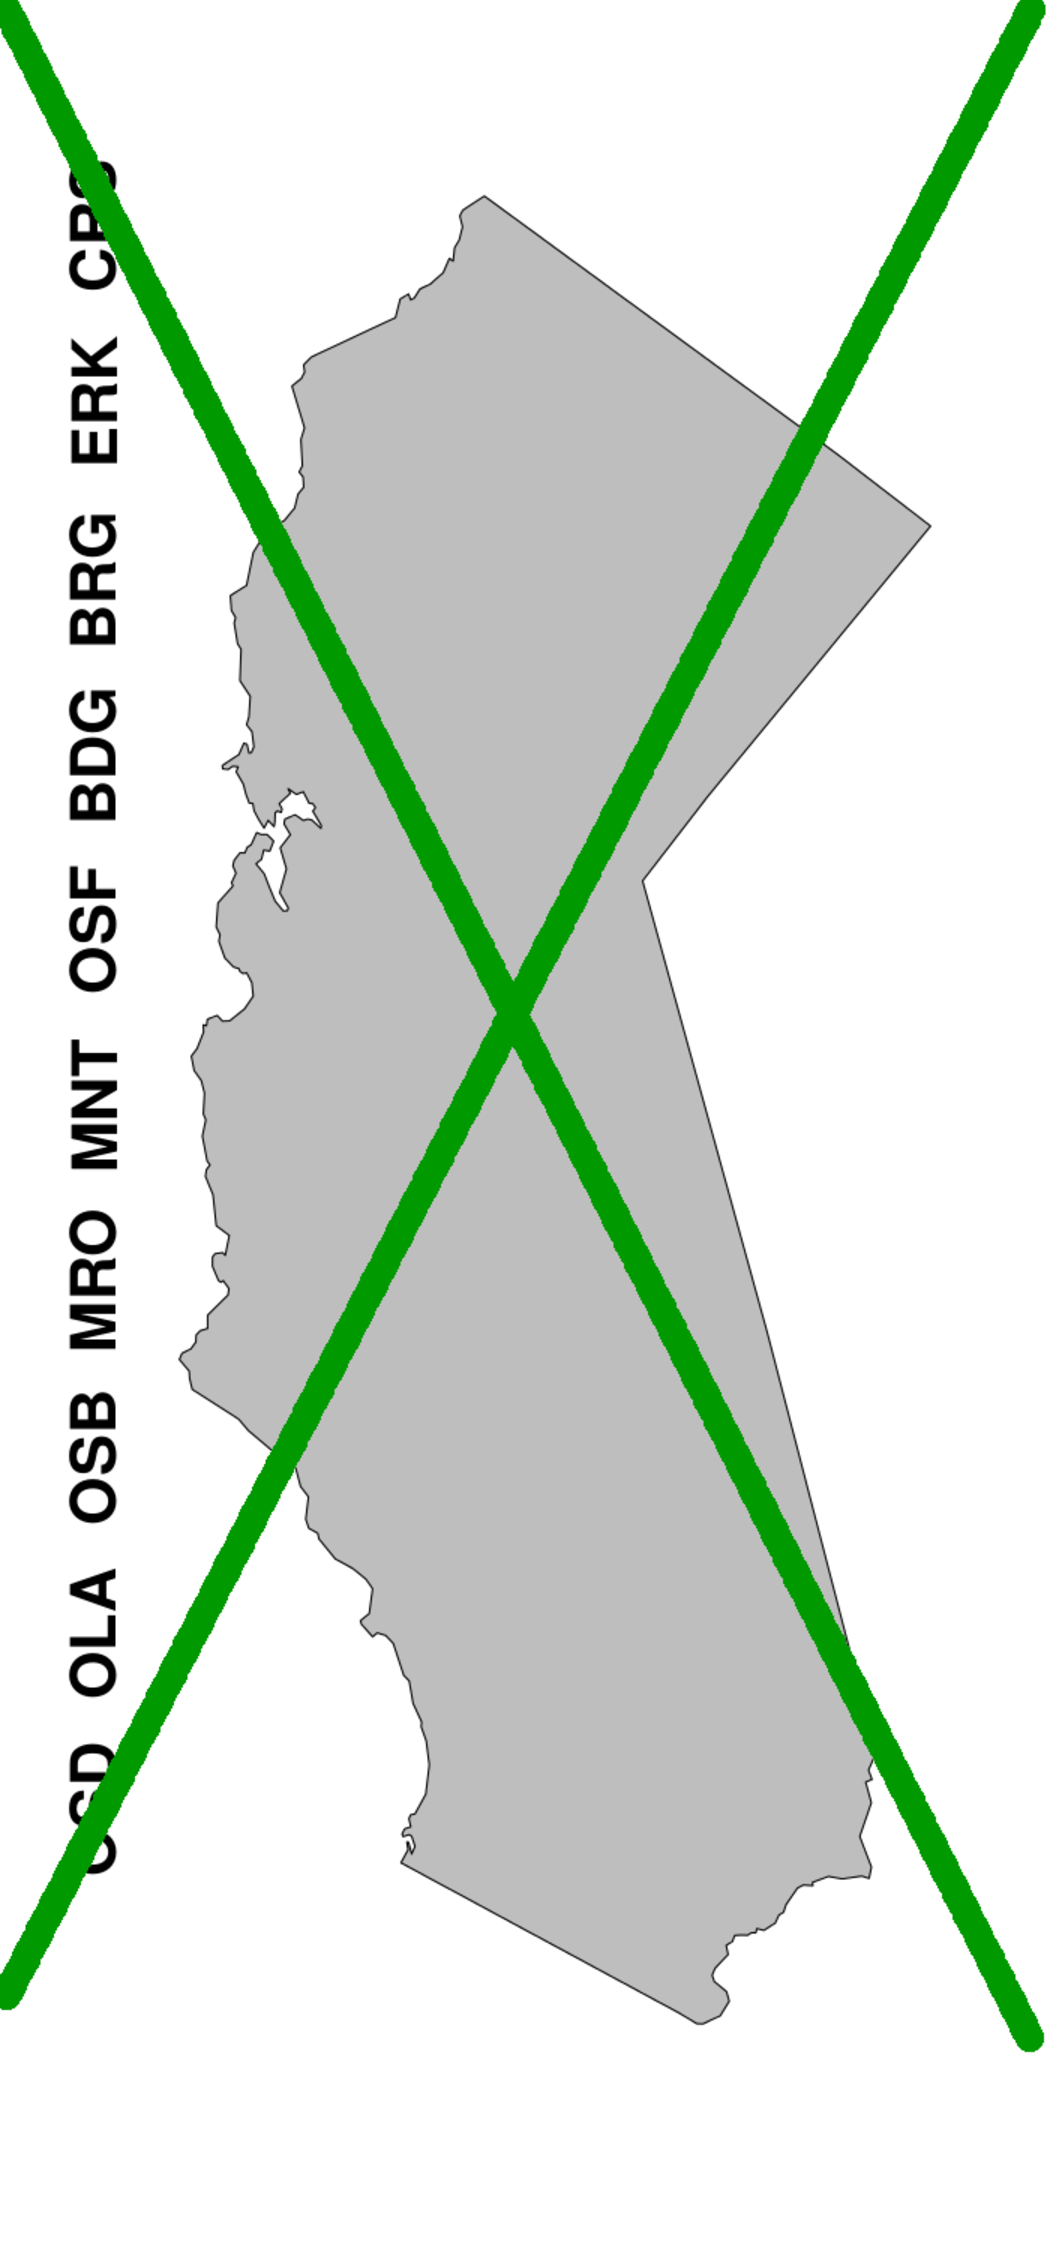
\includegraphics[width=0.91\textwidth]{../pictures/mapFullBlankNotGreen.pdf}
	\end{minipage}
	\begin{minipage}[h!]{0.19\textwidth}
	        %\hspace*{-0.25cm}
	        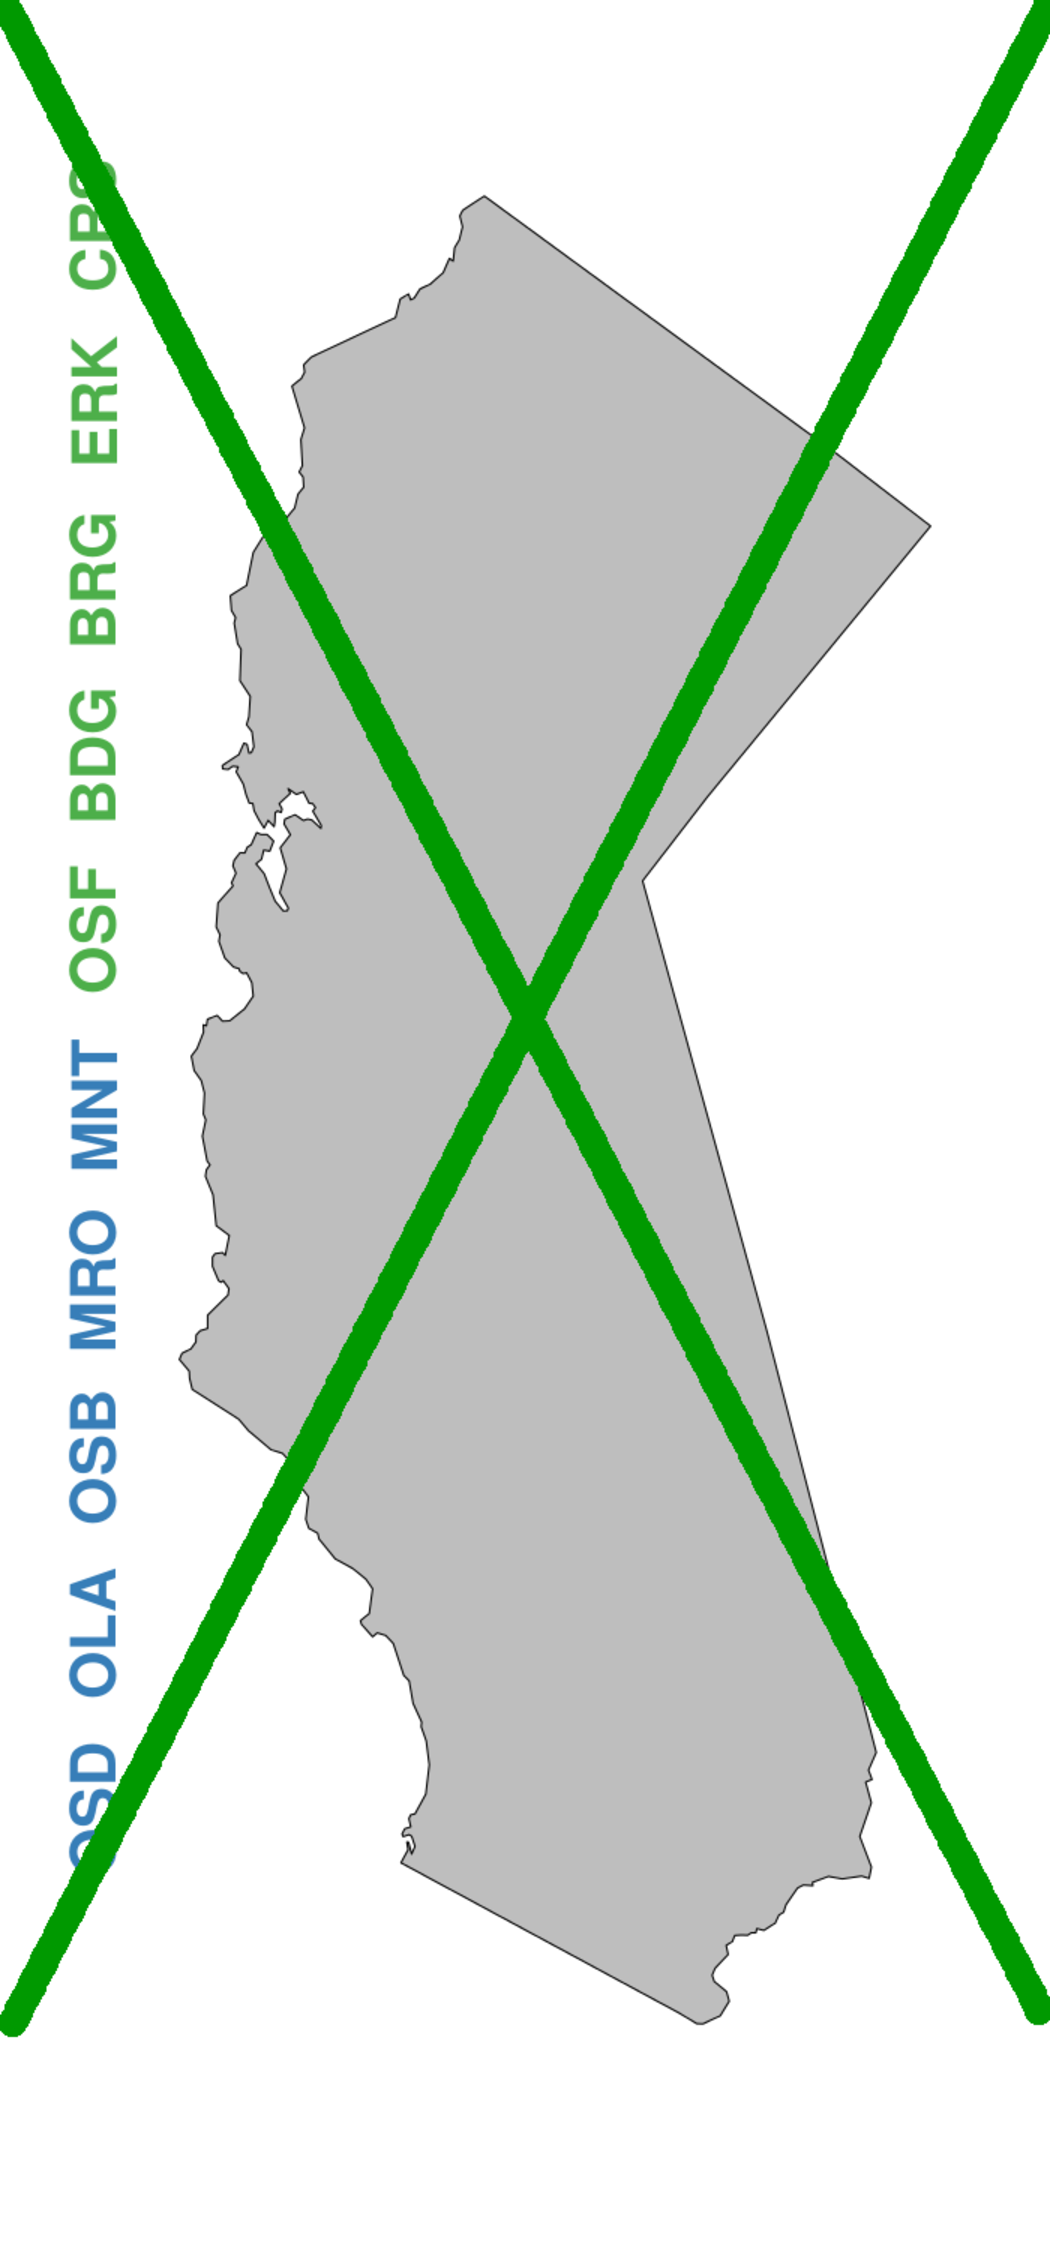
\includegraphics[width=0.91\textwidth]{../pictures/mapFullHalfHalfNotGreen.pdf}
	\end{minipage}
	\begin{minipage}[h!]{0.19\textwidth}
	        \hspace*{0.125cm}
	        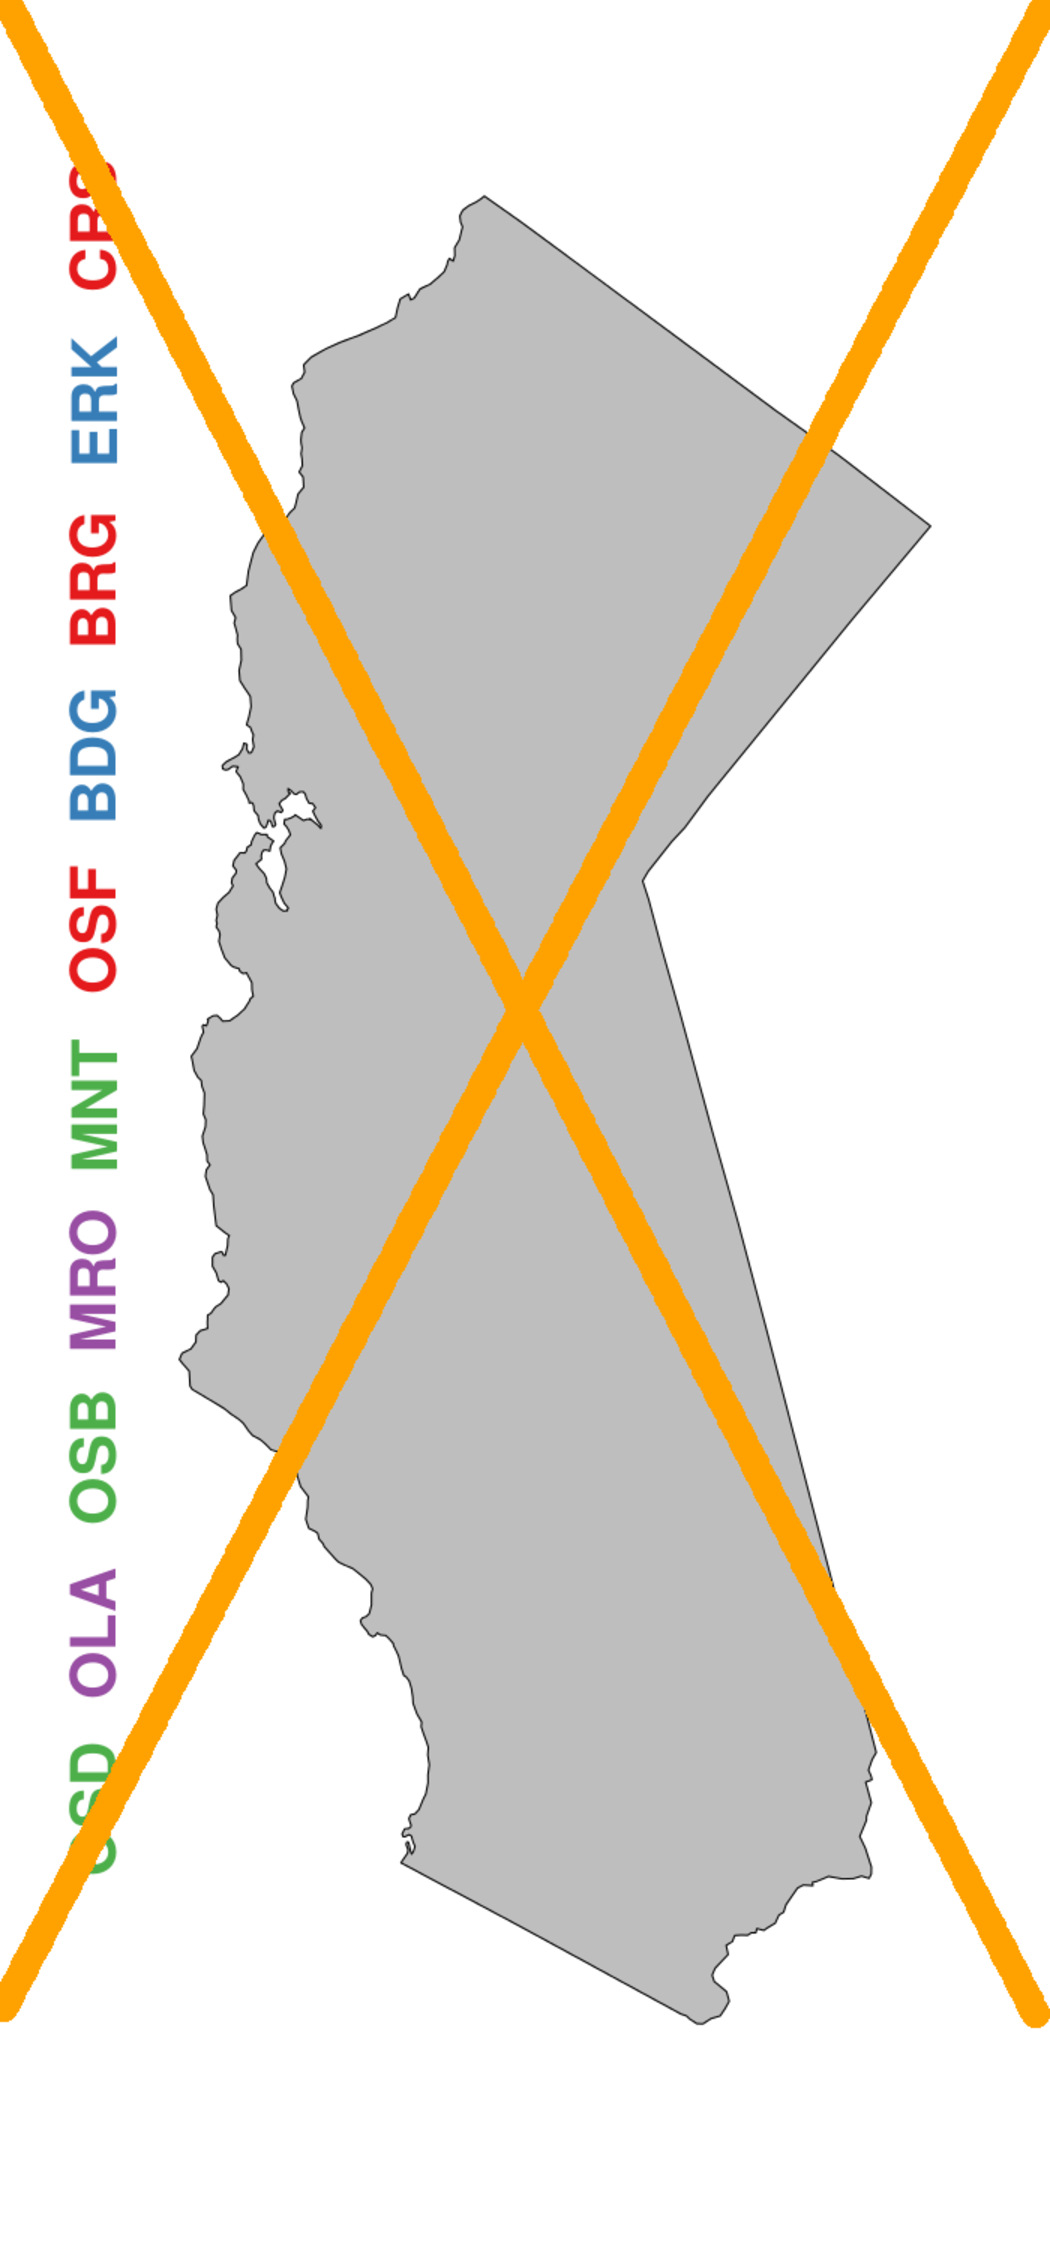
\includegraphics[width=0.91\textwidth]{../pictures/mapLeapFrogNotOrange.pdf}
	\end{minipage}
	\begin{minipage}[h!]{0.19\textwidth}
	        \hspace*{0.25cm}
	        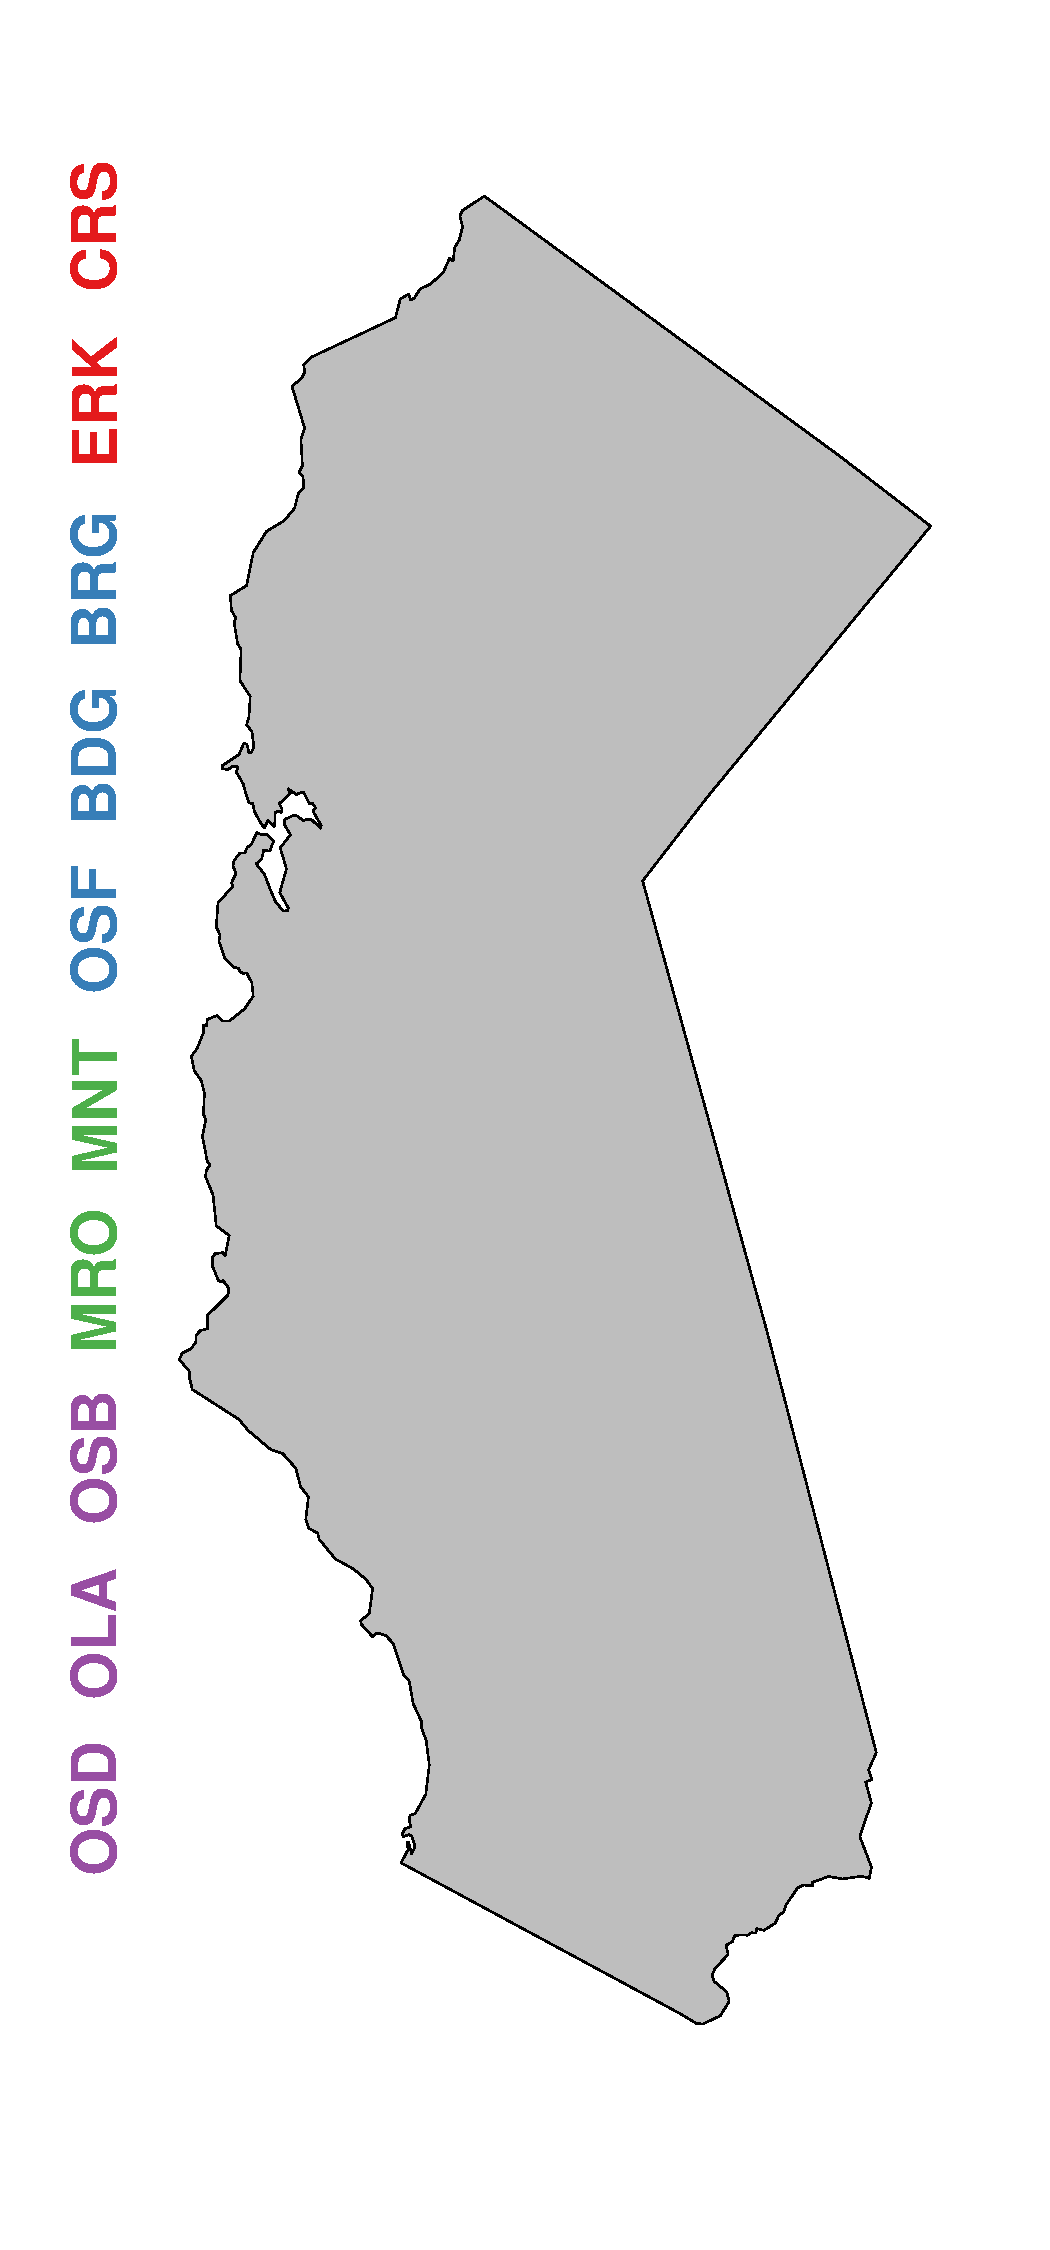
\includegraphics[width=0.91\textwidth]{../pictures/mapFullConcMend.pdf}
	\end{minipage}	
	\begin{minipage}[h!]{0.19\textwidth}
	        \hspace*{0.5cm}                %1.2
	        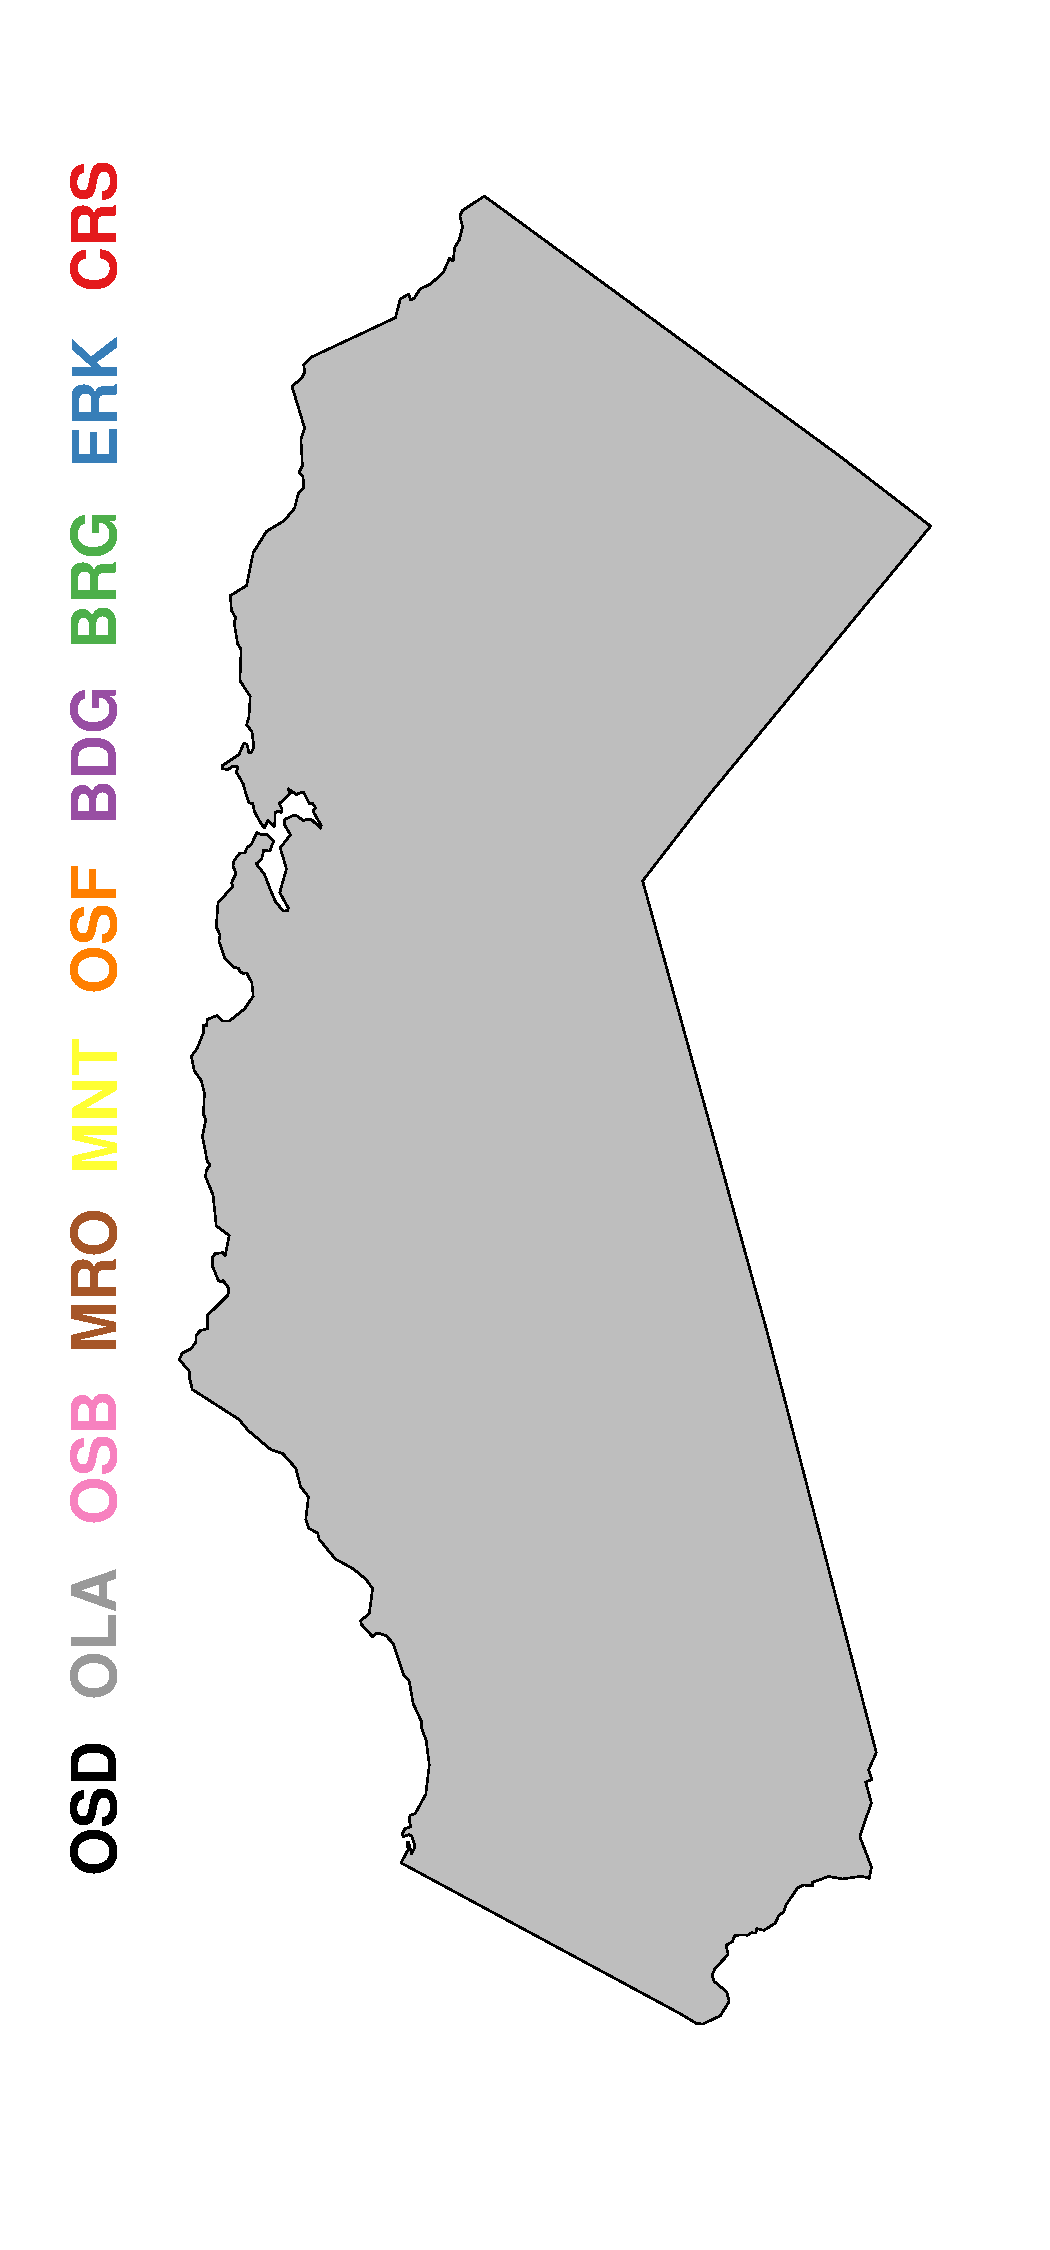
\includegraphics[width=0.91\textwidth]{../pictures/mapFullSparse.pdf}
	\end{minipage}
}

%
\headerbox{Group Bocaccio/Chili: 1983-1990}{name=colorTable,column=2,below=bma,span=1}{
	\resizebox{1\textwidth}{!}{
	\begin{tabular}{|c|c|c|c|c|c|}%|c|c|c|c|c|}
         \hline \multicolumn{6}{|c|}{MCAT 956} \\ \hline
         $\omega$&0.26&0.21&0.19&0.11&0.10\\ \hline %&0.08&0.00&0.00&0.00&0.00 \\ \hline
        CRS&\cellcolor[HTML]{E41A1C}&\cellcolor[HTML]{E41A1C}&\cellcolor[HTML]{E41A1C}&\cellcolor[HTML]{E41A1C}&\cellcolor[HTML]{E41A1C}\\ \hline %&\cellcolor[HTML]{E41A1C}&\cellcolor[HTML]{E41A1C}&\cellcolor[HTML]
        ERK&\cellcolor[HTML]{E41A1C}&\cellcolor[HTML]{377EB8}&\cellcolor[HTML]{E41A1C}&\cellcolor[HTML]{377EB8}&\cellcolor[HTML]{E41A1C}\\ \hline %&\cellcolor[HTML]{377EB8}&\cellcolor[HTML]{377EB8}&\cellcolor[HTML]
        BRG&\cellcolor[HTML]{377EB8}&\cellcolor[HTML]{4DAF4A}&\cellcolor[HTML]{377EB8}&\cellcolor[HTML]{4DAF4A}&\cellcolor[HTML]{377EB8}\\ \hline %&\cellcolor[HTML]{4DAF4A}&\cellcolor[HTML]{377EB8}&\cellcolor[HTML]
        BDG&\cellcolor[HTML]{377EB8}&\cellcolor[HTML]{4DAF4A}&\cellcolor[HTML]{377EB8}&\cellcolor[HTML]{4DAF4A}&\cellcolor[HTML]{377EB8}\\ \hline %&\cellcolor[HTML]{4DAF4A}&\cellcolor[HTML]{4DAF4A}&\cellcolor[HTML]
        OSF&\cellcolor[HTML]{4DAF4A}&\cellcolor[HTML]{4DAF4A}&\cellcolor[HTML]{377EB8}&\cellcolor[HTML]{4DAF4A}&\cellcolor[HTML]{377EB8}\\ \hline %&\cellcolor[HTML]{984EA3}&\cellcolor[HTML]{4DAF4A}&\cellcolor[HTML]
        MNT&\cellcolor[HTML]{4DAF4A}&\cellcolor[HTML]{984EA3}&\cellcolor[HTML]{4DAF4A}&\cellcolor[HTML]{984EA3}&\cellcolor[HTML]{4DAF4A}\\ \hline %&\cellcolor[HTML]{984EA3}&\cellcolor[HTML]{4DAF4A}&\cellcolor[HTML]
        MRO&\cellcolor[HTML]{4DAF4A}&\cellcolor[HTML]{984EA3}&\cellcolor[HTML]{4DAF4A}&\cellcolor[HTML]{984EA3}&\cellcolor[HTML]{4DAF4A}\\ \hline %&\cellcolor[HTML]{984EA3}&\cellcolor[HTML]{984EA3}&\cellcolor[HTML]
        OSB&\cellcolor[HTML]{984EA3}&\cellcolor[HTML]{984EA3}&\cellcolor[HTML]{4DAF4A}&\cellcolor[HTML]{FF7F00}&\cellcolor[HTML]{984EA3}\\ \hline %&\cellcolor[HTML]{FF7F00}&\cellcolor[HTML]{984EA3}&\cellcolor[HTML]
        OLA&\cellcolor[HTML]{984EA3}&\cellcolor[HTML]{FF7F00}&\cellcolor[HTML]{984EA3}&\cellcolor[HTML]{FF7F00}&\cellcolor[HTML]{984EA3}\\ \hline %&\cellcolor[HTML]{FF7F00}&\cellcolor[HTML]{984EA3}&\cellcolor[HTML]
        OSD&\cellcolor[HTML]{984EA3}&\cellcolor[HTML]{FF7F00}&\cellcolor[HTML]{984EA3}&\cellcolor[HTML]{FF7F00}&\cellcolor[HTML]{984EA3}\\ \hline %&\cellcolor[HTML]{FF7F00}&\cellcolor[HTML]{FF7F00}&\cellcolor[HTML]
	\end{tabular}	
	}
}

%
\headerbox{Results}{name=results,column=0,below=examples,span=2}{
	\vspace{-0.3cm}
	\begin{minipage}[h!]{0.49\textwidth}
                \hspace*{-0.2cm}
                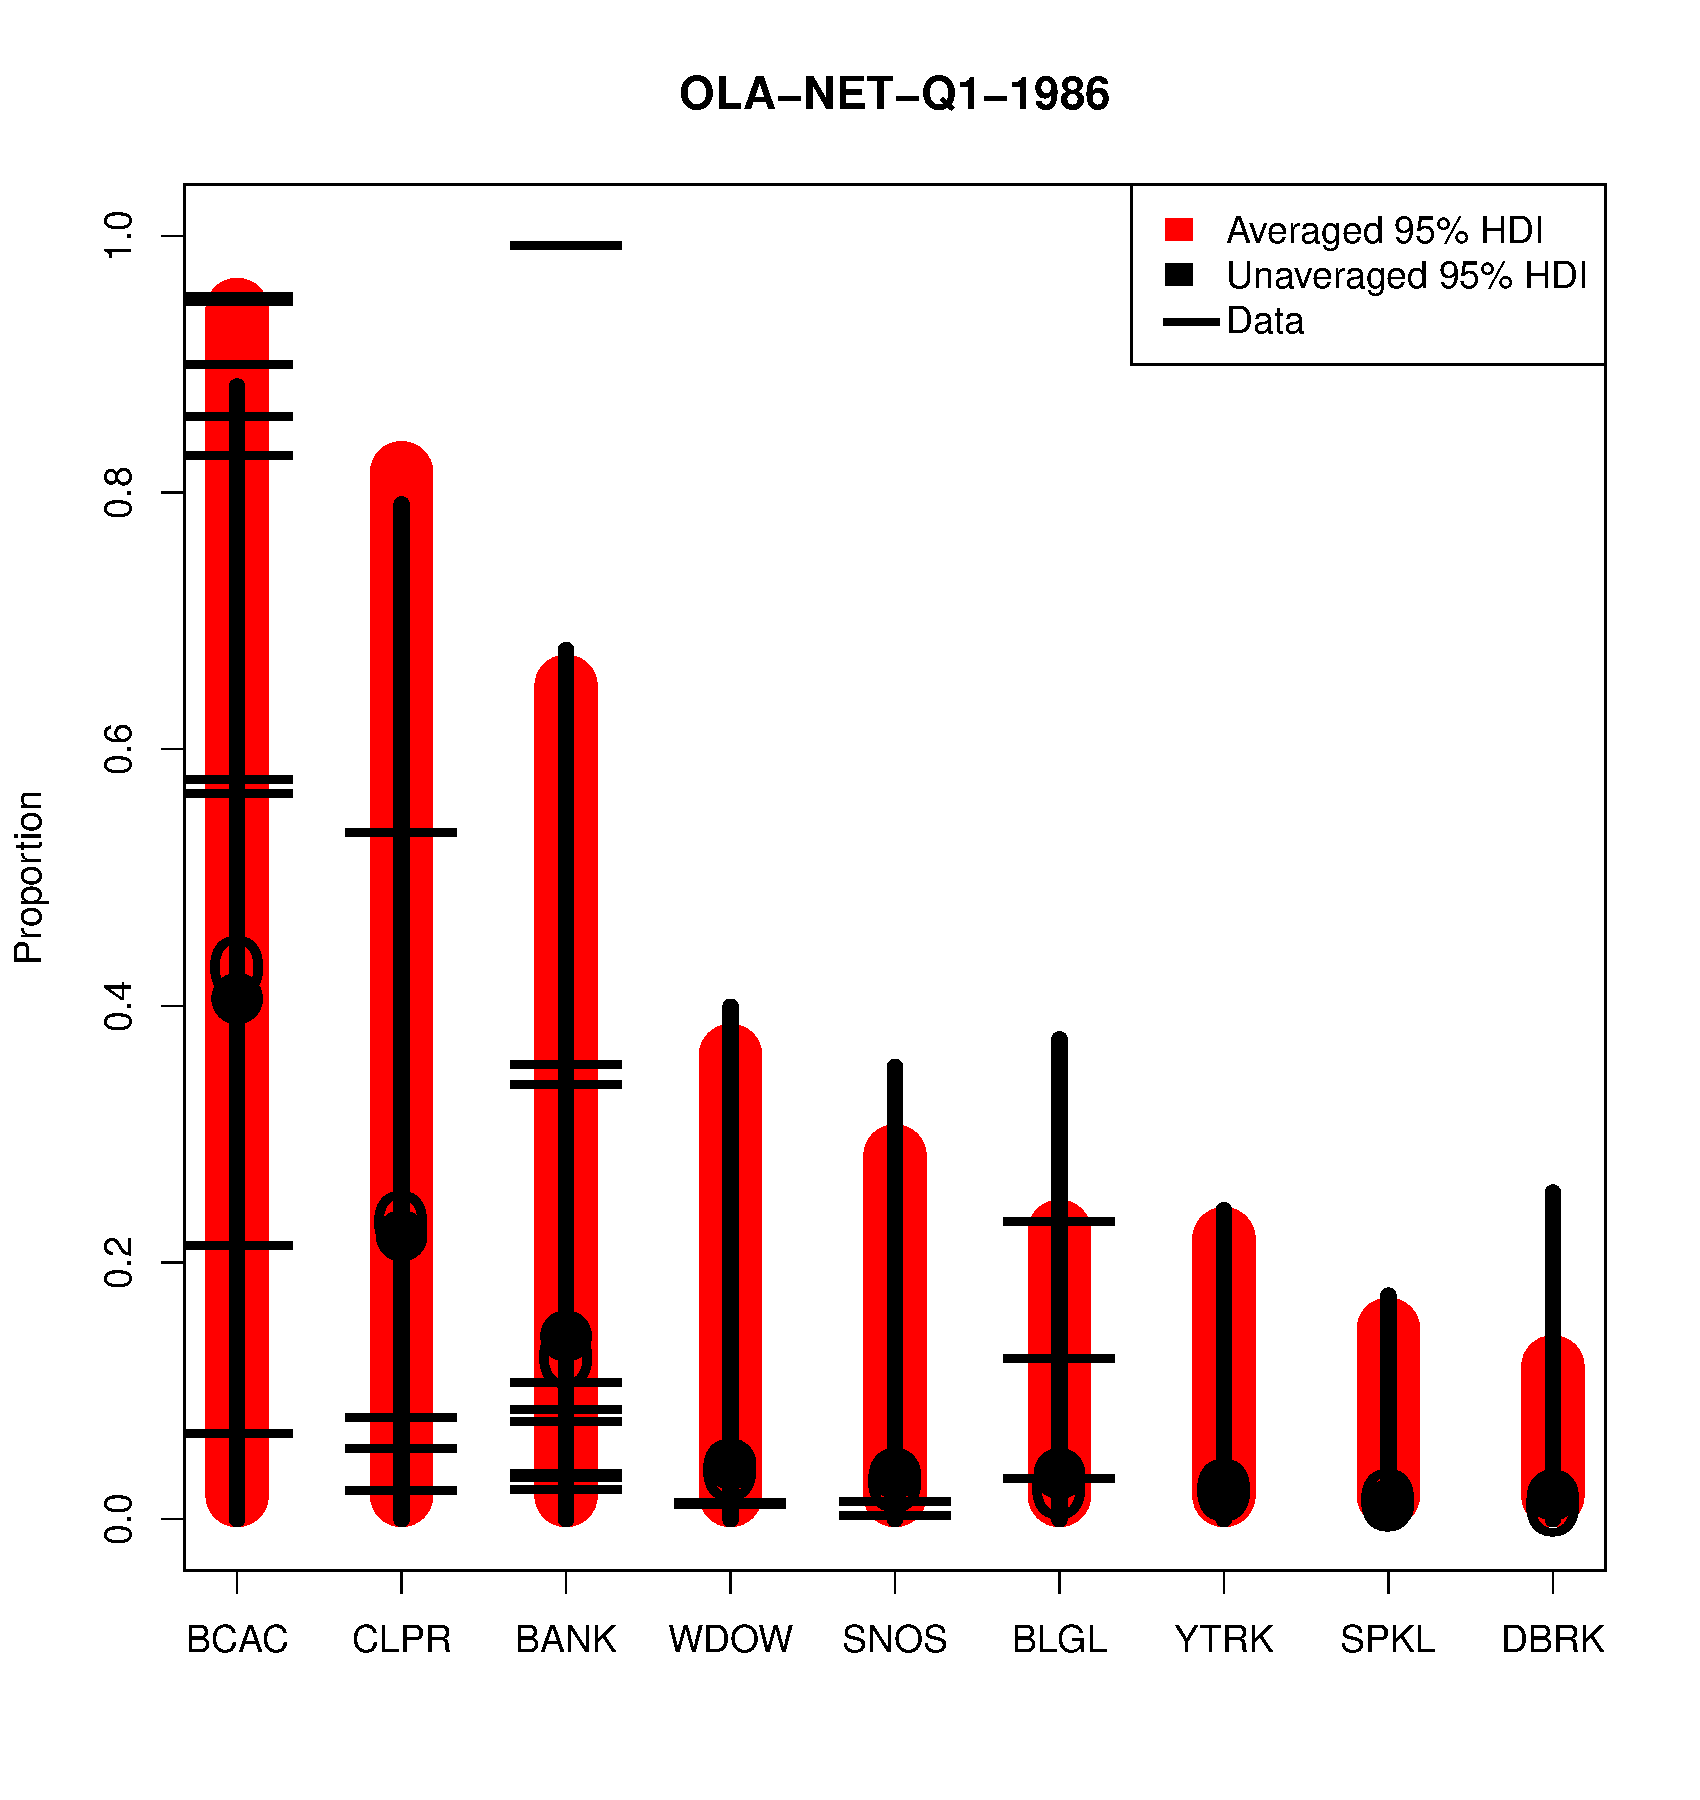
\includegraphics[width=1\textwidth, trim={0 1cm 0 0},clip]{../pictures/avgOrNotBox.pdf}
        \end{minipage}
        \begin{minipage}[h!]{0.49\textwidth}
		%\hspace*{-0.75cm}
		%\vspace{0.3cm}
		%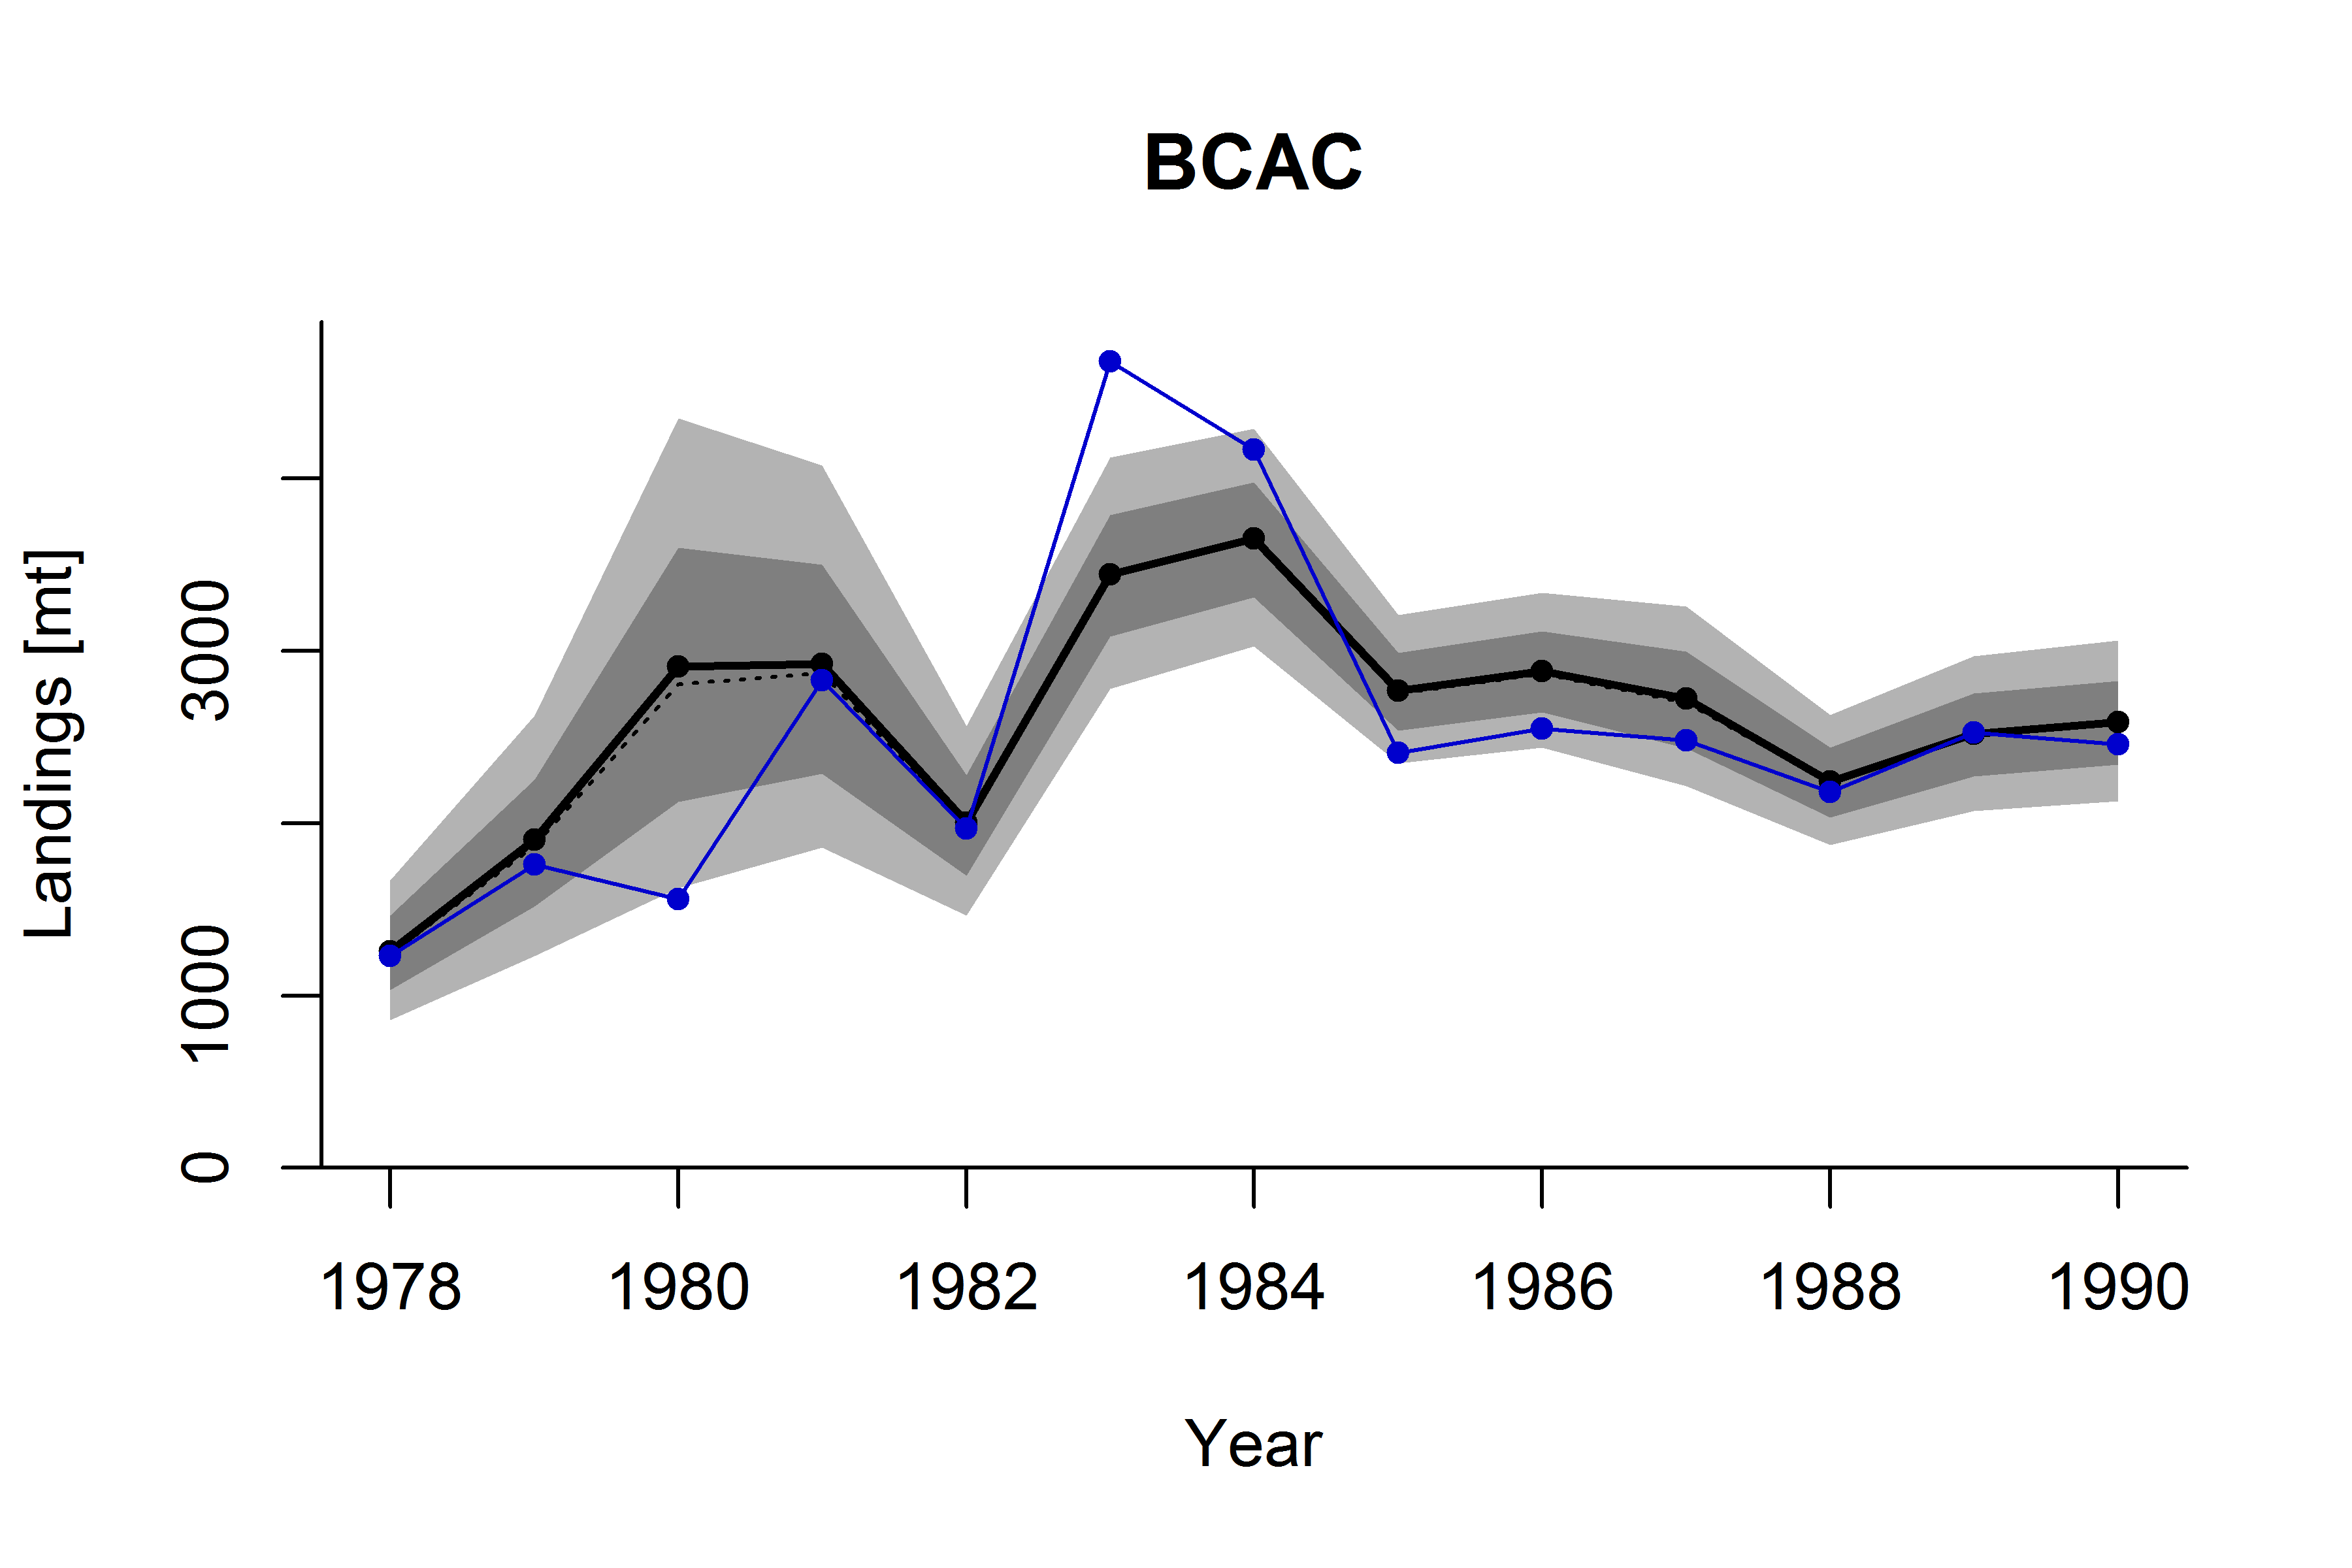
\includegraphics[width=1.1\textwidth, height=8cm]{../pictures/sp-yr/BCAC.png}
		\begin{minipage}[c]{0.49\textwidth}
		\hspace*{-1.5cm}
		\includegraphics[width=1.1\textwidth, height=3.5cm]{../pictures/sp-yr-gr/{trawl.BCAC}.png}
		%\end{minipage}
		%\begin{minipage}[c]{0.25\textwidth}
		\hspace*{-0.5cm}
		\includegraphics[width=1.1\textwidth, height=3.5cm]{../pictures/sp-yr-gr/{line.BCAC}.png}
		\end{minipage}
		\begin{minipage}[c]{0.49\textwidth}
		\vspace{-2.2cm}
		\hspace*{-1cm}
		\includegraphics[width=1.1\textwidth, height=3.5cm]{../pictures/sp-yr-gr/{gill_net.BCAC}.png}
		%\end{minipage}
		%\begin{minipage}[c]{0.25\textwidth}
		\vspace{-1.5cm}
		\hspace*{0.4cm}
		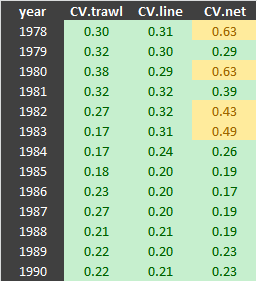
\includegraphics[width=0.7\textwidth]{../pictures/CVs_BCAC.png}
		\end{minipage}
        \end{minipage}
	(Left) Species composition predictions from the ensemble model, along side predictions from the base 
	model, and raw data from an example stratum in MCAT 956. %Model averaging has the effect of regularizing predictive intervals. 
	(Right) Grey regions show the BMA landings 80\% and 25\% intervals for BCAC by gear 
	from 1978-1990, current calcom estimates shown in blue, and nominal expansion shown in red.
	BMA CVs are shown in the bottom right.
	%It seems like this panel needs some word. I'm not sure yet which would be the best words, 
	%but these words can serve as a place holder. I really don;t know how many words I need. I 
	%think I need more words. Nooooo moooooorre words. I need more damn wooords.
}

%
\headerbox{Conclusion}{name=conclusion,column=2,below=colorTable,span=1}{
	$~$\\
	A Bayesian model-based method for speciating commercial landings shows promise. 
	BMA adds robustness to models by effectively integrating over modeling uncertainties.
	\\\\
	\underline{\textbf{Achievments of the Bayesian Approach:}}
	\begin{itemize}
	\item Model Overdispersion
	\item Robust Uncertainty Estimation
	\item Mechanisms for Pooling
	\item Out-of-Sample Predictions
	\end{itemize}
	$~$\\
	\underline{\textbf{Future Directions:}}
	\begin{itemize}
	\item Explore Additional Random Effects
	\item Possible Multivariate Likelihoods
	\item Dirichlet Process Models
	\end{itemize}
	\vspace{0.15cm}
}

%
%%
%\headerbox{6. Conclusion}{name=conclusion,column=0,below=results,span=3}{
%
%}

%\headerbox{2. Pharmacophore model}{name=model,column=0,below=introduction,span=1}{
%
%To describe a molecule, DeCAF substitutes its functional groups with pharmacophoric points (hence the "F" in the algorithm's name).
%Points are organised into an undirected graph.
%Lengths of the edges in the graph represents the number of bonds between pharmacophoric points.
%
%%\begin{center}
%%    \includegraphics[width=\linewidth]{phar}
%%\end{center}
%%%\vspace{-2pt}
%}
%
%
%\headerbox{3. Similarity measure}{name=mcs,column=0,below=model,span=1}{
%
%To measure similarity of two molecules or to combine them into one model, DeCAF first finds their \textbf{maximum common substructure (MCS)}.
%To provide fast, but accurate method for solving MCS problem, we combined Generic Match Algorithm (GMA) \cite{xu1996gma} with backtracking algorithm proposed by Yiqun Cao \cite{cao2008maximum}.
%
%Here we present comparison of molecules with similar and with different structures.
%DeCAF scores and \textbf{Tanimoto coefficient (Tc)} values are shown in red and black, respectively.
%%\begin{center}
%%    \includegraphics[width=\linewidth]{sim}
%%\end{center}
%}
%
%\headerbox{4. Applications}{name=screen,span=2,column=1,below=introduction}{ % To reduce this block to 1 column width, remove 'span=2'
%
%DeCAF is a versatile tool with many possible applications.
%It allows to compare two molecules or more complex models created from sets of ligands.
%Our method can be used to align multiple ligands and find crucial pharmacophoric features in a set of active compounds.
%Pharmacophore models can help in database screening for molecules with desired properties.
%DeCAF is also suitable for comparing entire sets of ligands, e.g. to analyse properties of proteins in drug repositioning process.
%
%%\vspace{-5pt}
%%\begin{center}
%%    \includegraphics[width=0.85\linewidth]{screen}
%%\end{center}
%}
%
%
%\headerbox{5. DeCAF vs. SEA}{name=sea,span=2,column=1,below=screen}{ % To reduce this block to 1 column width, remove 'span=2'
%
%%\begin{wrapfigure}{l}{0.3\textwidth}
%%    \vspace{10pt}
%%    \begin{center}
%%        \includegraphics[width=\linewidth]{class}
%%    \end{center}
%%    %\vspace{-145pt}
%%\end{wrapfigure}
%
%% We tested DeCAF in 35 case studies taken from the DUD-E database, to evaluate its power to discriminate between active and inactive molecules.
%% We used DeCAF as a classifier and compared it to the SEA (Similarity Ensemble Approach) algorithm \cite{keiser2007relating}.
%% To compare sets of ligands, we adapted the approach used in SEA, replacing Tc by DCAF.
%% We prepared datasets as shown in the left diagram.
%% Then, we tested both classifiers calculating ROC AUC values for every target (below).
%We tested DeCAF in 35 diverse targets taken from the DUD-E database, to evaluate its power to classify molecules as active or inactive.
%We compared DeCAF to the renowned \textbf{SEA (Similarity Ensemble Approach)} algorithm \cite{keiser2007relating}, which uses Tc as a similarity measure.
%Dataset preparation steps are shown on the left diagram.
%Comparison results (\textbf{ROC AUC} values for each receptor) are shown below.
%% Please ask me about details.
%
%%\hspace{0pt}\includegraphics[width=0.95\linewidth]{res}
%
%}
%
%
%\headerbox{6. Conclusions}{name=conclusion,column=1,below=sea,span=2,above=bottom}{
%% DeCAF is a chemoinformatical tool that can be helpful in ligand-based drug design.
%% It provides a comprehensive molecule description and a fast algorithms for comparing and aligning multiple ligands.
%We proved that DeCAF is a significant improvement over the SEA algorithm, a popular method for comparing sets of ligands.
%\begin{boenumerate}\compresslist
%    \item DeCAF gives better results for 23 out of 35 receptors.
%    \item For targets with easily separable active and inactive datasets, SEA and DeCAF give similar results.
%    \item In cases in which SEA fails to identify active molecules, our method performs substantially better.
%\end{boenumerate}
%% It can be also used in other [procedures], such as database screening or drug repositioning.
%% DeCAF is written in Python and freely available at \textbf{\color{darkgreen}http://bitbucket.org/marta-sd/decaf}. 
%}
%
%
%\headerbox{7. References}{name=references,column=0,span=1,below=mcs,above=bottom}{
%
%
%%\small % Reduce the font size in this block
%\renewcommand{\section}[2]{\vskip 0.05em} % Get rid of the default "References" section title
%%\nocite{*} % Insert publications even if they are not cited in the poster
%
%
%\bibliographystyle{unsrt}
%\bibliography{poster} % Use sample.bib as the bibliography file
%}

\end{poster}

\end{document}

